\section{Methodology for Testing FBs}
\label{sec::methodology}
Our proposed approach for cross-platform FB testing is suitable for a test-driven development process, as well as for testing existing implementations. It involves specifying tests, executing tests within an IDE, generating the portable test application, as well as executing these tests on all relevant RTEs. A test application that is compliant with IEC~61499 can be ported to RTEs of various vendors. The approach is visualised in Figure~\ref{fig::methodology} as a step-by-step approach using the generated test cases of our running example (Section~\ref{sec::running_example}). In the following, we describe each step of the process in detail. We describe the envisioned development process based on our running example. %Detailed transformation rules for the generation of IEC~61499 software will be described in Section~\ref{sec::transformationrules}.

\subsection{Test-driven Development of FBs}
The following steps describe a test-driven development process. For testing existing FB libraries, the process starts directly at step 4, as the implementation is already complete. In this case, test cases will be generated semi-automatically from the implementation to reduce the effort.

\subsubsection{Creating a new Function Block type (FBT)}
Reusable functionality should be encapsulated in an FB. This involves specifying the input/output events and data inputs/outputs. %Unless the developer adheres to a test-driven development (TDD) process, the internal behaviour of the FB is implemented as well. 
For the running example, this involves defining the interface of the calculation FB.

\subsubsection{Specify test cases as service sequence models} Specification models are defined.
   %In this step, the test cases for the FB are specified as service models. There are two approaches to this:
   % \begin{enumerate}
   % \item Manually defining Service Sequences: The test cases are manually defined as service sequences, representing the expected behaviour of the FB under different scenarios.
  %  \item  Recording Service Sequences using the interpreter: Alternatively, the test cases can be recorded using the interpreter, which 
 %   \end{enumerate}
In the running example, a service model with two sequences is provided to define the test scenarios for the FB (cf. Figure~\ref{fig::methodology}, step 2). The service model specifies the expected event occurrences, as well as the input values (\texttt{DI1} and \texttt{DI2}) and the expected output value (\texttt{DO1}) for each test case.  
The scenario of \texttt{test1} is triggered upon arrival of an event at the input \texttt{REQ}. The purpose of \texttt{test1} is to describe the FB behaviour by checking whether it correctly returns 19 when given input values of 5 and 7. 
Additionally, \texttt{test2} aims to evaluate the FB behaviour for an edge case, as one value will be out of range (i.e., \texttt{DI2:=INT\#1001}). We expect that no addition is performed, and no output events are sent (cf. second sequence in step 2). 
Where output data values are expected, they are specified together with the output event. %it can be determined whether the FB behaves as intended.
% TODO BIANCA adds the figures to this sequence

    \subsubsection{Implement desired functionality of the FB type}
    When following a TDD process, the functionality of the FB is implemented at this stage. The specified tests can be used for iteratively evaluating the correctness. For instance, the implemented behavior of an FB can be analysed using model interpreters to receive rapid feedback on any changes. 
    For the running example, we assume that the limit check of DI2 was not yet implemented. This scenario is illustrated in step 3 of Figure~\ref{fig::methodology}. When the test cases are executed using a model interpreter \cite{wiesmayr2021}, the feedback shows that an unexpected event occurrence (i.e., CNF) has been output by the FB under test. 
    By comparing the actual output with the expected output for each test case, the implemented FB behaviour is evaluated automatically.
    As a result, the transition condition of the state diagram can be updated to include the missing check for \texttt{DI2<=1000}. Afterwards, evaluating the service sequence is successful.

\subsection{Testing Implemented FBs}
    After an FB has been developed, it needs to be evaluated in an RTE. While manual testing is feasible on all existing RTEs, automating the process allows to reduce the development time and effort. Hence, the following steps describe the process of model-based testing by generating an IEC~61499-based test application from the test specification.

\setcounter{subsubsection}{3}
   \subsubsection{Defining (additional) test cases for the implemented FB}
    Especially when validating the behavior of an FB in different platforms, creating test cases for additional corner cases may be useful. Even when a test-driven development approach is followed, a comprehensive test suite may not be available. Using a model interpreter and its accompanying execution framework~\cite{wiesmayr2021} allows recording additional test cases based on specified events and/or data inputs. This also allows adding test suites to existing implementations.  Step 4 in Figure~\ref{fig::methodology} shows the dialogue for recording a service sequence where DI1 is out of range. The resulting graphical diagram is added to the FB type specification and is shown on the right. Developers have to manually check whether the result matches the expected behaviour of the developed FB. Recorded tests can serve as regression tests, as they capture the actual behaviour of an executed FB. This can ensure that an FB is evaluated comprehensively during model evolution. 
  
\subsubsection{Generate test application for specified test cases}
    Once the implementation has been completed, the correct real-time behavior of an FB has to be evaluated in a run-time environment. The test application ensures that developers do not need to manually interact with an FB and observe the outputs. Hence, various components are required for issuing test signals, which can be automatically generated. They are visualized in step 5 of Figure~\ref{fig::methodology} and described as follows:
    \begin{itemize}
        \item \textbf{(A) Test signal generator:} This FB generates the input signals based on the service model and supplies the required events and data to the FB under test (REQ, DI1, DI2). It also notifies the test application of the expected output events (CNF or none). Additionally, it provides the expected output values (DO1), which are set in algorithms. 
        \item \textbf{(B) Matcher:} This FB compares the execution results of the FB under test with the expected results that are provided by the test signal generator. 
        \item \textbf{(C) Multiplexer: } The next FB forwards the result (ERROR, SUCCESS) of each test case (i.e., service sequence) to the output, together with the name of the executed test case. This helps developers to identify the faulty test case if there are any problems. 
        \item \textbf{(D) Test application composite: } A composite FB encapsulate the test application so that it can be easily deployed to an RTE. All components are interconnected to provide a simple interface. Developers can run each test case by triggering the respective events. An additional event pin ``run\_all'' is provided to execute all test cases sequentially based on a single event trigger. This functionality is handled by an additional FB which initiates these further test cases. 

    \end{itemize}
        Some of the components (e.g., the matcher) also require a timer to wait for the results of the FB under test, thus, ensuring that no unexpected event outputs are detected. As a result, timer FBs are included in the test application.
        Note that the test signal generator, the FB under test, and the matcher are instantiated once per test case. This ensures that the internal state of these components does not affect further test cases. The FBs are guaranteed to initiate the execution from the START-state. As all FBs for the test application require an internal state, they are realized as Basic FBs. Although Figure~\ref{fig::methodology} visualizes the test environment for a Basic FB (i.e., the running example), any kind of FB can serve as the FB under test. Only the interface definition and the service model are required. This also means that application parts can be tested as long as they are integrated into an FB.

Based on the results provided in \cite{Testing_Midhun,biancaMidhunETFAwip}, we derived transformation rules for creating test code from service models. We implemented these rules in Eclipse 4diac~\cite{eclipse4diac}, which provides an open source IDE for IEC 61499-based software.
\begin{figure*}
    \centering
    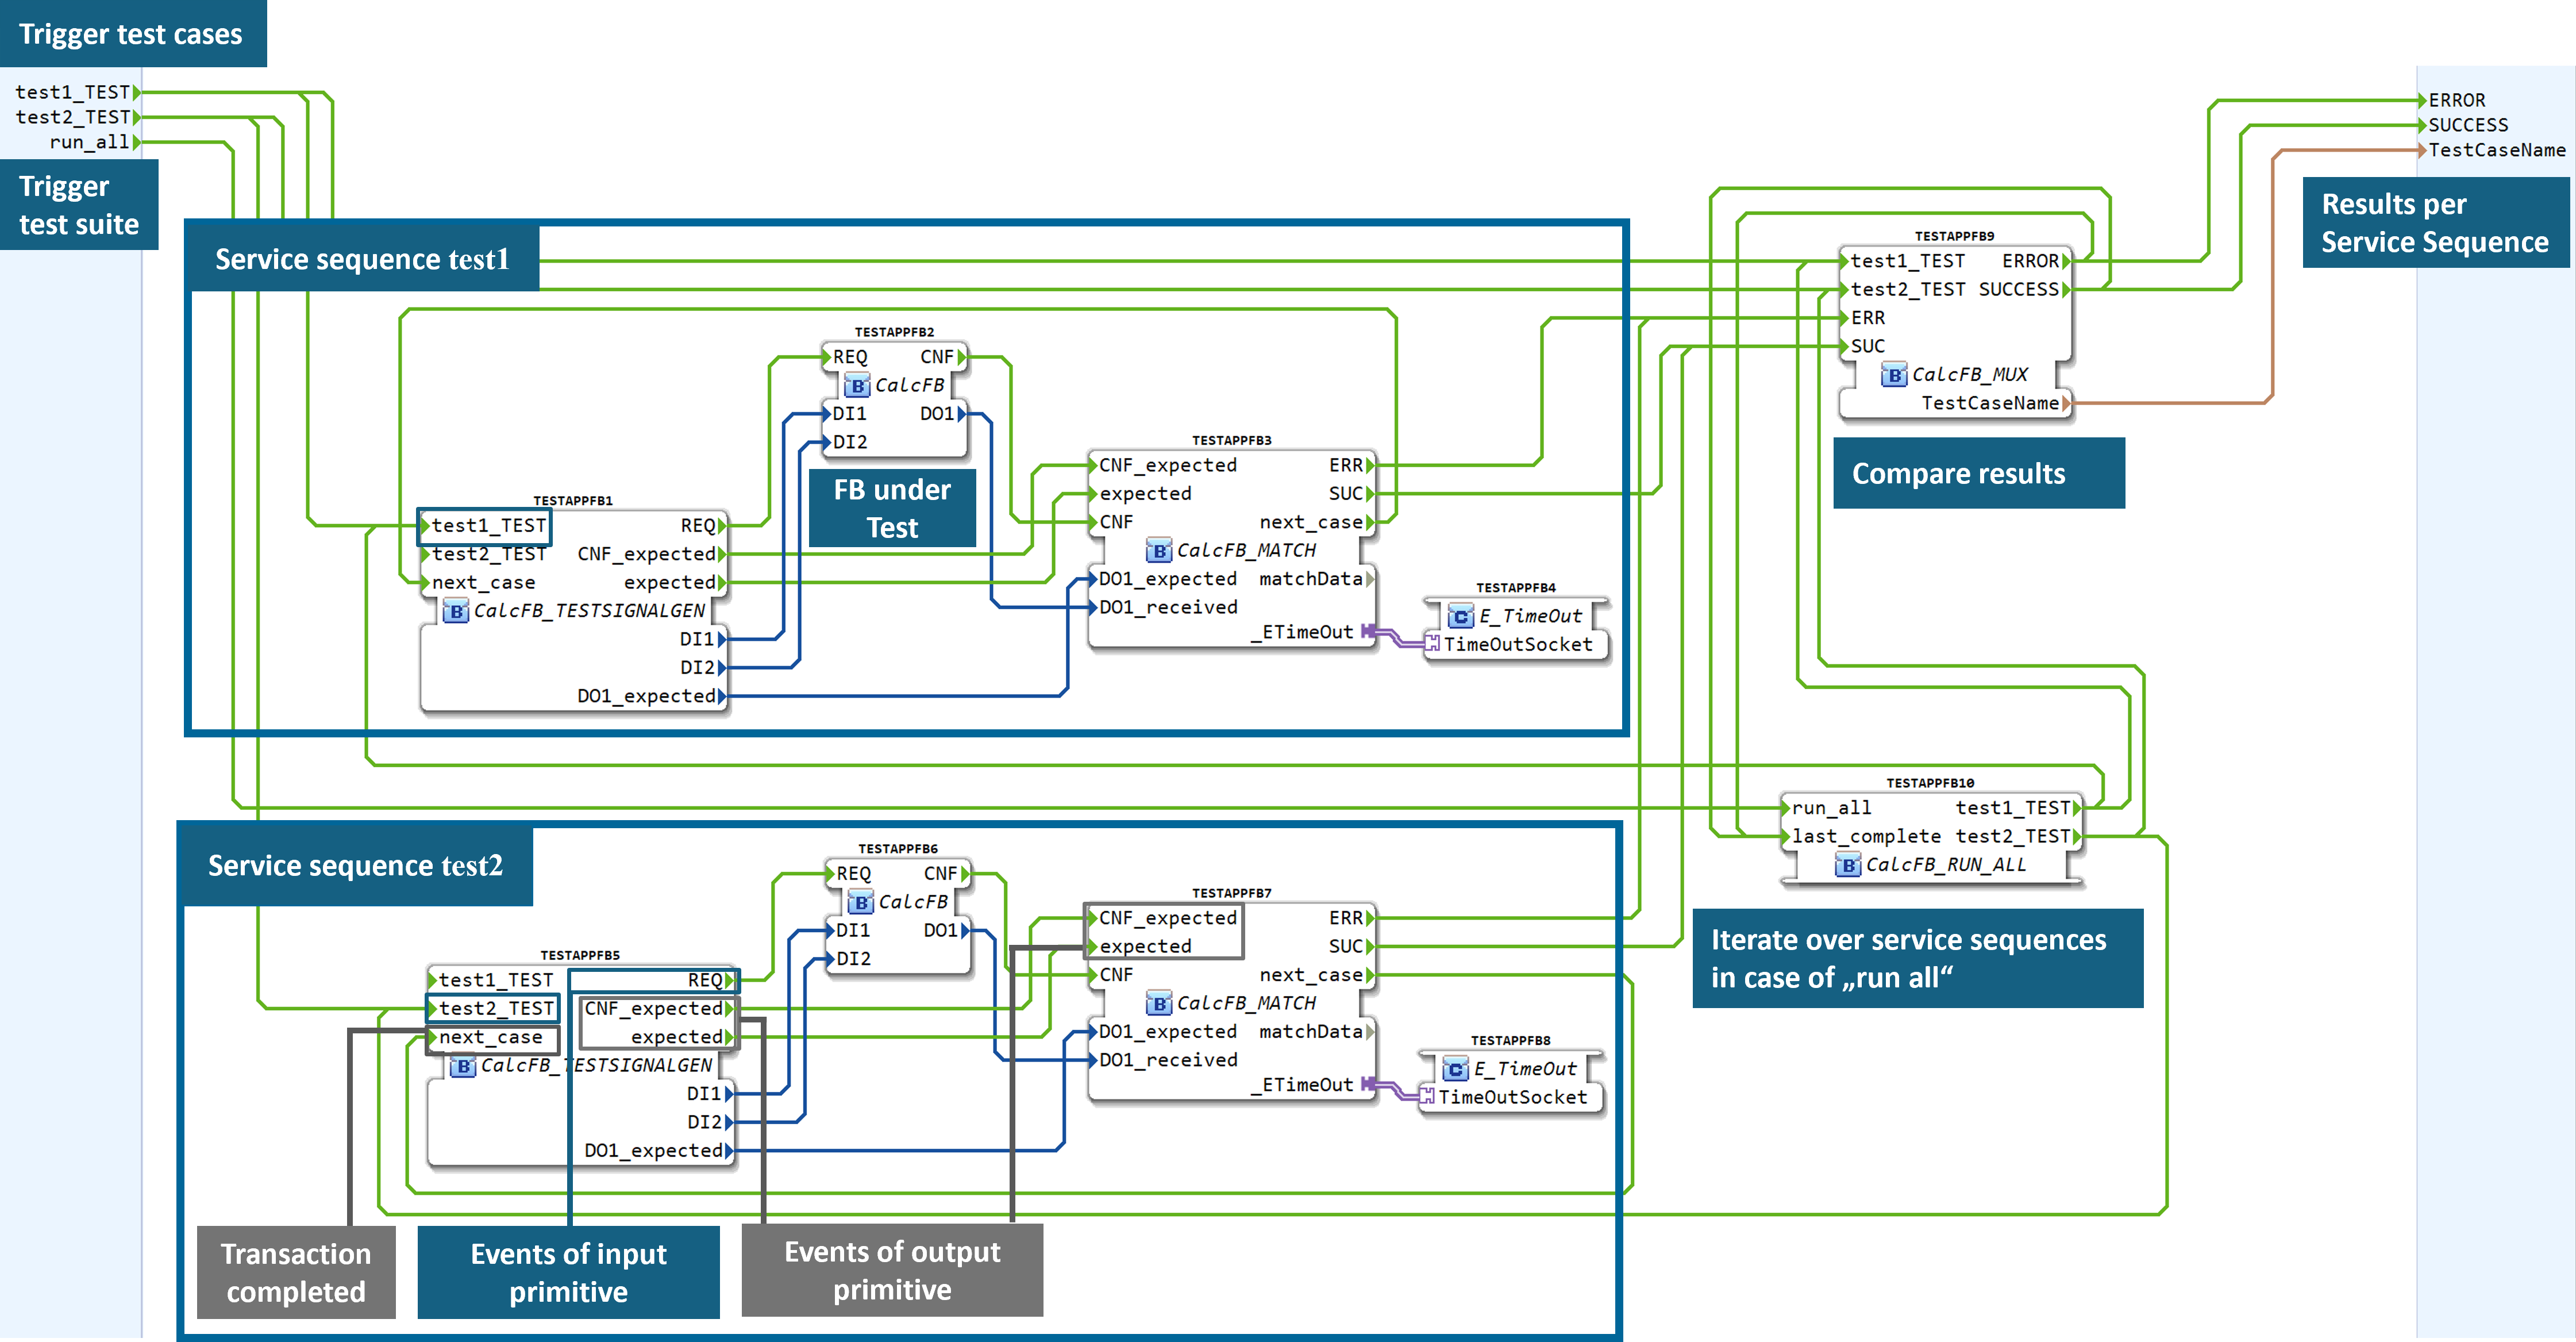
\includegraphics[width=\linewidth]{OJIES_2024/Figures/generation_rules.png}
    \caption{Test application generated for two service sequences of the running example. Relevant regions are highlighted including their relation to the service model.}
    \label{fig::testapp}
\end{figure*}

\begin{itemize}
        \item  A \textbf{service model} serves as the test suite and includes one or more service sequences. A single test application is generated for the whole service model. 
        
        \item Each \textbf{service sequence} serves as one test case. We need one event input per test case in the test application FB, which will trigger the execution of this test. We include its name in the event pin to relate the parts of the test application with the respective service sequences. Once the service sequence was completed, an ERROR or SUCCESS event is issued, together with the name of the service sequence. A service sequence can consist of several service transactions, which define the flow of events along the sequence. 
         
         \item Each \textbf{service transaction} is comprised of an input primitive (ingoing arrow) and any number of output primitives (outgoing arrows). The service transactions are processed one after another. An event issued by the matcher (nextCase) indicates that a transaction has been completed.
        
        \item The \textbf{input primitive} describes the event that initiates a transaction. 
        The test signal generator FB has to issue the input event specified in a transaction. They are supplied to the FB under test via the respective connections together with the associated data. As a result, the test signal generator FB requires one output pin (events and data) for each input pin of the FB under test. 
        
        \item The \textbf{output primitives} describe the event(s) that is/are caused by the input event.
        The test signal generator FB issues an event indicating all output events that are part of a test sequence. They are supplied to the FB under test via the respective connections together with the associated data. As a result, the test signal generator FB requires one output pin (events and data) for each input pin of the FB under test. The matcher FB receives information about the expected events and data values from the signal generator FB. It compares them with the events and data received from the FB under test.
\end{itemize}


\subsubsection{Port test application to other platforms}
The presented development approach is fully supported in 4diac~IDE~\cite{eclipse4diac}. Although service sequences are defined in the standard, they are not fully supported in other tools. Also the model execution framework for evaluating FBs is provided in 4diac~IDE. Hence, the test application is generated in 4diac~IDE following the notation of the IEC~61499 standard, and is then ported to other platforms. Manual effort may be required for importing FBs developed in one IDE to other vendors \cite{cheng_pang_portability}.

\subsubsection{Execute Tests in All Relevant RTEs}
The generated test application (i.e., the composite FB), is deployed to and executed on different RTEs. The behaviour and output results of the FB are evaluated manually in each RTE.



